\documentclass[../main.tex]{subfiles}
\graphicspath{{\subfix{../img/}}}

\begin{document}

% \thispagestyle{empty}
% \etocignoretoctocdepth % of course, if we want to see something in local TOC...
% \etocsettocstyle{\subsection*{\contentsname}}{}
% \localtableofcontents
% \newpage
% \setcounter{page}{1}

%%%%%%%%%%%%%%%%%%%%%%%%%%%%%%%%%%%%%%%%%%%%%%%%%%%%%%%%%%%%%%%%%%%%%%%%%%%%%%%%%
\section{Mathematical and Computational Background} \label{sec:math_background}

As discussed in Section \ref{sec:sleep_and_r5_network}, R5 neurons exhibit variety of response properties under different experimental conditions: they show tonic firing during day, $\sim1$Hz bursting at night and after sleep deprivation, and low-frequency spiking (potentially mediated by Ca$^{2+}$ channels) following the blockade of Na$^+$ channels. The biological mechanisms underlying these responses and the transition between them are poorly understood. This section reviews the background on bursting neurons from mathematical and computational perspectives and concludes with suggestions for modeling the behavior of R5 neurons.

%%%%%%%%%%%%%%%%%%%%%%%%%%%%%%%%%%%%%%%%%%%%%%%%%%%%%%%%%%%%%%%%%%%%%
\subsection{Models of Bursting Neurons}

\subsubsection{Preface} \label{subsubsec:bursting_models_preface}

As discussed in Section \ref{subsubsec:bio_burst_onset_offset}, at the level of ion channels, different ionic mechanisms can underlie bursting, depending on which ionic currents are responsible for initiation and termination of the bursts.
However, irrespective of the specific ionic channels involved, resting and spiking states, as well as transitions between them, can exhibit different characteristics across different models. The examples of bursting neurons in Figures \ref{fig:ionic_basis_for_slow_fast_bursting}
and \ref{fig:example_forced_intrinsic_bursters} illustrate the case when the resting
state is a stable equilibrium and the spiking state is a limit cycle attractor. However,
generally, the resting state can also be a limit cycle attractor (not shown here).
As the electrophysiological recordings of R5 neurons do not show subthreshold oscillations
at the resting state, this case will be omitted in this chapter. The case when the resting state
is a stable equilibrium is referred to as \textbf{\textit{'point-cycle burster'}}
\parencite{izhikevichNEURALEXCITABILITYSPIKING2000}, and will be the main focus in the following.

Bursting is commonly modeled as a dynamical system consisting of two - \textbf{fast and slow subsystems}, with the fast system having two states - spiking and resting, while the slow system slowly modulates the transition of the fast subsystem between the two states. 
In other words, modulation of the slow variable causes transitions between the states in the fast subsystem. Mathematically, such transitions can be analyzed using bifurcation theory \parencite{izhikevichDynamicalSystemsNeuroscience2006,izhikevichNEURALEXCITABILITYSPIKING2000,golombContributionPersistentNa2006}.

\begin{figure}[!t]
    \centering
    \includegraphics[width=0.85\linewidth]{../img/modeling_r5/examples/intrinsic_vs_forced_burster.png}
    \caption[Forced vs intrinsically bursting neurons]{
        Forced vs intrinsically bursting neurons. Examples of model neurons bursting due to time-varied external input (a) and intrinsic
        properties (b). Adapted from \parencite{izhikevichDynamicalSystemsNeuroscience2006}, with modifications.
    }
    \label{fig:example_forced_intrinsic_bursters}
\end{figure}

%%%%%%%%%%%%%%%%%%%%%%%%%%%%%%%%%%%%%%%%%%%%%%%%%%%%%%%%%%%%%%%%%%%%%%%%%%%%%
\subsubsection{Classification} \label{subsubsec:math_bursting_classification}

Models of the bursting neurons can be classified according to the modeling approach, response to the external input, or the dynamical characteristics of the transitions between spiking and resting states. The current section provides an overview of these classification frameworks. Classification based on the dynamical characteristics will be discussed in more detail in Section \ref{subsec:bifurcation_analysis}.

%%%%%%%%%%%%%%%%%%%%%%
\vspace*{0.3cm}
\noindent\textbf{Modeling approach}

Based on the modeling approach, they can be classified into \textbf{phenomenological} (e.g. proposed by Izhikevich \parencite{izhikevichSimpleModelSpiking2003,izhikevichNEURALEXCITABILITYSPIKING2000}, or Hindmarsh-Rose \parencite{wangGenesisBurstingOscillations1993}) and \textbf{conductance-based} (first proposed by Hodgkin and Huxley \parencite{hodgkinQuantitativeDescriptionMembrane1952}) models. One of the most widely-used phenomenological models for bursting is the one proposed by Izhikevich \parencite{izhikevichSimpleModelSpiking2003}, governed by the following system of differential equations:
\begin{align}
    \frac{dv}{dt}&=0.04 v^2 + 5v + 140 - u + I \label{eq:izhikevich_model_v} \\
    \frac{du}{dt}&=a(bv-u) \label{eq:izhikevich_model_u}
\end{align}
where $v$ is the membrane potential, and $u$ represents a recovery variable acting as negative feedback on the membrane potential, accounting for activation of K$^+$ and inactivation of Na$^+$ channels, and $I$ represents the external current. The spikes are generated by manually resetting variables when $v$ reaches predefined threshold $v_{thr}$:
\begin{equation*}
    \left\{
    \begin{array}{l}
    v \leftarrow c \\
    u \leftarrow u + d
    \end{array}
    \right.
    \quad \text{if } v \geq v_{\text{thr}}
\end{equation*}
By changing the dimensionless parameters $a$, $b$, $c$, and $d$ the model can reproduce a variety of spiking behaviours. However, such phenomenological models are not detailed enough to investigate effects of ion channels, as they do not account for the intrinsic mechanisms of activity generation.

On the other hand, conductance-based models describe the interactions between membrane potential and ionic currents, thereby providing insights into the underlying biological mechanisms responsible for observed neuronal activity patterns. Since the aim of this thesis is to understand which biological mechanisms may contribute to the generation of diverse activity patterns observed in R5 neurons, conductance-based models will be the primary focus of the following work.

Furthermore, neurons can be modelled using \textbf{single-} or \textbf{multicompartment} approaches.
In general, the distribution and/or concentration of the ion channels varies across different parts of the neuron, such as soma, dendrites, and axon, with some ion channels expressed in particular regions \parencite{destexheDendriticLowthresholdCalcium1998,gunayDistalSpikeInitiation2015}.
In addition, neuronal morphology has been shown to enhance robustness to parameter variations and significantly influence neuronal computations, including synaptic integration, as well as initiation and propagation of action potential \parencite{destexheDendriticLowthresholdCalcium1998,gunayDistalSpikeInitiation2015,cuntzOneRuleGrow2010}.
Multicompartment models account for these spatial variations by modeling different neuronal compartments and interactions between them. In contrast, single-compartment models assume a uniform distribution of ion channels and represent neurons as a single, uniform unit. Nevertheless, single-compartment models have been found to be sufficient for replicating many experimental observations \parencite{wangMultipleDynamicalModes1994,golombContributionPersistentNa2006,destexheDendriticLowthresholdCalcium1998,liuMultipleConductancesCooperatively2008,vickstromTTypeCalciumChannels2020}.
Although multicompartment models are more biologically plausible and can better reproduce experimental data, single-compartment models are more computationally efficient (see also discussion) \parencite{destexheDendriticLowthresholdCalcium1998}.


%%%%%%%%%%%%%%%%%%%%%%
\vspace*{0.3cm}
\noindent\textbf{Response to the external input}

Generally, any model neuron that spikes can also burst under modulation of
time-dependent external input $I(t)$ \parencite{izhikevichDynamicalSystemsNeuroscience2006}
(\textbf{\textit{forced burster}}, Fig. \ref{fig:example_forced_intrinsic_bursters}a).
However, a neuron can also burst intrinsically under constant input due to the interplay
between ionic currents mediated by ion channels present in the membrane of the neuron
(\textbf{\textit{intrinsic burster}}, Fig. \ref{fig:example_forced_intrinsic_bursters}b).
Although it is not known whether R5 neurons are intrinsic bursters or not
\parencite{raccugliaNetworkSpecificSynchronizationElectrical2019}, as \gls{swa}
is thought to be generated at the level of R5 \parencite{raccugliaNetworkSpecificSynchronizationElectrical2019},
in the current work, it will be assumed that R5 neurons exhibit bursting behaviour
due to intrinsic properties, rather than via time-varied external input (refer to Section \ref{sec:sleep_and_r5_network} for details on the underlying biological motifs).

\begin{figure}[!t]
    \centering
    \includegraphics[width=0.85\linewidth]{../img/modeling_r5/examples/classification_of_intrinsic_bursters.png}
    \caption[Classification of intrinsically bursting neurons by neuro-computational features]{
        \textbf{Classification of intrinsically bursting neurons by neuro-computational features.}
        Adapted from \parencite{izhikevichDynamicalSystemsNeuroscience2006}, with modifications.
        Electronic version of the figure and reproduction permissions
        are freely available at \url{www.izhikevich.com}.
    }
    \label{fig:classification_intrin_burst}
\end{figure}

Bursting in neurons can arise through various mechanisms and is often classified based on the type of external current under which the neuron exhibits bursting behaviour. Models that burst due to a neuron's intrinsic properties can be categorized into one of the following classes: (1) \textbf{tonic bursting}, where the neuron generates repetitive bursts in response to a constant depolarizing current, (2) \textbf{phasic bursting}, where a single burst followed by a quiescent state is observed near the onset of a constant depolarizing current, (3) \textbf{rebound bursting}, where a burst is elicited following termination of hyperpolarizing step current, and (4) \textbf{inhibition-induced bursting}, where neuron exhibits periodic bursting during the application of hyperpolarizing external current \parencite{izhikevichDynamicalSystemsNeuroscience2006,izhikevichWhichModelUse2004}. The examples of each type of bursting are depicted in Figure \ref{fig:classification_intrin_burst}.

%%%%%%%%%%%%%%%%%%%%%%
\vspace*{0.3cm}
\noindent\textbf{Classification based on dynamical characteristics}

As it was mentioned in Section \ref{subsubsec:bursting_models_preface}, bursting is commonly modelled as an interaction between fast and slow subsystems, with the fast subsystem having two states (spiking and resting), and the slow subsystem governing transition between the two.

Within the framework of a fast-slow system, bursting can be categorized into two classes depending on the mechanism governing transitions between the two states of the fast subsystem - \textbf{hysteresis-loop} and \textbf{slow-wave} bursting (Figure \ref{fig:slow_wave_and_hysteresis_bursting}). One key difference between the two is that slow-wave bursting requires the slow system to be at least 2-dimensional to generate oscillations,
whereas the hysteresis-loop bursting can occur with a single slow variable. Additionally, in slow-wave bursting, the transition between spiking and resting states occurs due to reversing the direction of the slow variable (Figure \ref{fig:slow_wave_and_hysteresis_bursting}, left). In contrast, hysteresis-loop bursting exhibits more complex dynamics - the system remains in a spiking or resting state until the specific threshold is crossed. Reversing the direction of the slow variable is insufficient to induce the transition. This distinguishes the hysteresis loop from slow-wave bursting, where the slow subsystem itself drives periodic transitions between the two states.

It is worth noting that, in case of the slow-wave bursting, according to the textbook-definition \parencite{izhikevichNEURALEXCITABILITYSPIKING2000,izhikevichDynamicalSystemsNeuroscience2006}, the slow variable (e.g. $u$ in Equations \ref{eq:izhikevich_model_v}-\ref{eq:izhikevich_model_u}) evolves (relatively) independently of the fast subsystem. However, it does not imply that the slow subsystem is always autonomous, or that it always has a limit-cycle attractor. In some models, feedback from the membrane potential (e.g. \cite[p. 356]{izhikevichDynamicalSystemsNeuroscience2006}) or from variables of the fast subsystem (e.g. \cite[p. 1201]{izhikevichNEURALEXCITABILITYSPIKING2000}) is required to generate bursting behaviour.

\begin{figure}[!t]
    \centering
    \includegraphics[width=0.95\linewidth]{../img/2_mathematical_overview/slow_wave_and_hysteresis_bursting.png}
    \caption[Slow wave and hysteresis-loop bursting]{
        \textbf{Slow wave and hysteresis-loop bursting.}
        Adapted from \parencite{izhikevichDynamicalSystemsNeuroscience2006}, with modifications.
    }
    \label{fig:slow_wave_and_hysteresis_bursting}
\end{figure}


% %%%%%%%%%%%%%%%%%%%%%%%%%%%%%%%%%%%%%%%%%%%%%%%%%%%%%%%%%%%%%%%%%%%%%
% \subsubsection{Fast-slow Subsystems}

% \begin{figure}[!t]
%     \centering
%     \includegraphics[width=0.85\linewidth]{../img/2_mathematical_overview/fast_slow_system_example.png}
%     \caption[Example of fast-slow decomposition]{
%         \textbf{Example of fast-slow decomposition}.
%         Adapted from \parencite{izhikevichDynamicalSystemsNeuroscience2006}.
%         \textcolor{red}{Text}
%     }
%     \label{fig:example_fast_slow_decomposition}
% \end{figure}

%%%%%%%%%%%%%%%%%%%%%%%%%%%%%%%%%%%%%%%%%%%%%%%%%%%%%%%%%%%%%%%%%%%%%
\subsection{Bifurcation Analysis} \label{subsec:bifurcation_analysis}

Bifurcation analysis is a powerful tool to investigate the behaviour of
a dynamical system. Specifically, how the given system switches between
different states when one or multiple parameters (referred to as \textbf{bifurcation parameters})
are varied. By definition, bifurcation is a qualitative change in a system's topological structure that occurs when its parameters cross a bifurcation (or, critical) point \parencite{kuznetsovElementsAppliedBifurcation2023}.
% As it will be evident throughout this section, the choice of the bifurcation parameter is crucial and depends on what aspects of the system one aims to investigate.

Within the framework of the fast-slow subsystems with a single slow variable one can consider the slow variable as a bifurcation parameter and investigate how changing the value of that variable affects the state of the fast subsystem: for what values are the fast subsystem at rest, or spiking state, and how does transition between these states occur. Thus, when the mechanism of bursting is investigated,
one can divide the question into two parts: 1) how is the burst initiated?, and 2) how is the burst terminated? In the previous section, cellular mechanisms of these questions were summarized. In the current section, the same questions are approached from the perspective of mathematical analysis. Transition from resting (when the neuron does not fire action potentials) to spiking state is referred to as \textbf{bifurcation of equilibria}. Transition from spiking to resting state is referred to as \textbf{bifurcation of cycles} \parencite{izhikevichNEURALEXCITABILITYSPIKING2000,izhikevichDynamicalSystemsNeuroscience2006}.

Bifurcations are commonly divided into two classes: \textbf{local bifurcations} and \textbf{global bifurcations} \parencite{zhouBifurcation2013}. Local bifurcation occurs when the stability of a fixed point is changed when the bifurcation parameter is varied. Here, changes are confined within a small neighbourhood of a single fixed point and can be studied by linear stability analysis. In contrast, changes in the phase space in the case of global bifurcations occur on a larger scale (e.g. when two limit cycles collide with each other) and are harder to detect analytically \parencite{strogatzNonlinearDynamicsChaos2018}.
Bifurcations may be investigated using analytical methods or semi-analytical numerical tools (such as MATCONT \parencite{dhoogeMATCONTMATLABPackage2003} or AUTO \parencite{article}).

%%%%%%%%%%%%%%%%%%%%%%%%%%%%%%%%%%%%%%%%%%%%%%%%%%%%%%%%%%%%%%%
\subsubsection{Codim-1 bifurcations in planar fast-slow systems}

In bifurcation theory, \textbf{codimension 1} (or, \textbf{codim-1}) bifurcations occur when varying a single bifurcation parameter. If the system has one slow variable, one can study for what values of the slow variable the fast subsystem undergoes a state transition (from resting to spiking state, and vice versa).

Izhikevich studied codim-1 bifurcations in \textbf{planar systems}, where the fast subsystem is 2-dimensional \parencite{izhikevichNEURALEXCITABILITYSPIKING2000}. He identified $12$ relevant codim-1 bifurcations for the resting state, and $10$ for the spiking state. For a more detailed overview of the $120$ possible bifurcation pairs, the readers are referred to Table 4 in \parencite{izhikevichNEURALEXCITABILITYSPIKING2000}.

As it was discussed in Section \ref{subsubsec:bursting_models_preface}, generally, the fast subsystem may or may not exhibit oscillations at the resting state. The system that does not show oscillations at the resting state of the fast subsystem was referred to as a point-circle burster. Out of the above-mentioned $120$ bifurcation pairs, $36$ exhibit point-circle bursting, out of which $16$ can occur in planar systems.
The corresponding bifurcations of equilibria and cycles are given in Tables \ref{tab:bifurcations_equilibria} and \ref{tab:bifurcations_cycles}. Each bifurcation type has distinct properties and implications for the system's dynamics. 
In the following, possible bifurcations for point-circle bursting in planar systems will be summarized. Although the fast subsystem may undergo more than one bifurcation, and the list of possible onset and/or offset bifurcations may extend with increasing dimensionality of the system,
investigation of simpler, lower-dimensional systems provides valuable insight into the fundamental mechanisms of bursting. See also Section \ref{subsubsec:spiking_to_bursting_bifurcation} for the bifurcation analysis of one of the models implemented in this thesis — specifically, the model proposed by Wang \parencite{wangMultipleDynamicalModes1994}.

%%%%%%%%%%%%%%%%%%%%%%%%%%%%%%
\vspace*{0.3cm}
\noindent\textbf{Bifurcation of Equilibria}

\begin{table}[t!]
    \centering
    \begin{tabular}{|c||c|c|c|c|}
        \hline
        Bifurcation of Equilibria & Frequency & Amplitude \\ 
        \hline
        \hline
        Fold* & nonzero & fixed  \\
        Saddle-node on Invariant Cycle (SNIC)** & zero ($\sqrt{\lambda}$) & fixed \\
        Supercritical Hopf & nonzero & zero ($\sqrt{\lambda}$) \\
        Subcritical Hopf & nonzero & arbitrary \\
        \hline
    \end{tabular}
    \caption[Bifurcations of Equilibria of Fast Subsystem]{Bifurcations of Equilibria of Fast Subsystem
    (adapted from \parencite{izhikevichNEURALEXCITABILITYSPIKING2000} with modifications). *Also called saddle-node}
    \label{tab:bifurcations_equilibria}
\end{table}

Bifurcation of equilibria occurs when the stable fixed point loses its stability. Within the framework of a fast-slow system, the stable fixed point refers to one of the fast subsystems,
and the bifurcation happens when the slow variable passes through the critical value. Table \ref{tab:bifurcations_equilibria} summarizes the possible bifurcations of equilibria for point-circle bursting neurons.

\textbf{Fold} (or, \textbf{\gls{sn}}) \textbf{bifurcation} occurs when stable and unstable fixed points collide and annihilate each other. The example is illustrated in Figure \ref{fig:example_bifurcations_subhb_sn_sh_snic}A, which describes the bifurcations of the fast subsystem for one of the bursting neuron models from \parencite{franciRobustTunableBursting2018}. The black line represents the stable (solid) and unstable (dashed) fixed points of the fast subsystem, which depend on the value of the slow variable (here, $m_{KCa}$). For large values of $m_{KCa}$, the fast subsystem is in equilibrium. By reducing the value of the slow variable, two unstable fixed points appear, one of them colliding with the stable fixed point of the fast subsystem (\gls{sn}). As at that critical point of $m_{KCa}$, the stable fixed point is annihilated, the trajectory is drawn toward a different attractor of the dynamical system, in this case - stable limit cycle (the solid blue lines indicate the minimal and maximal values of the membrane potential during oscillations).

\textbf{\gls{snic}} bifurcation, depicted in Figure \ref{fig:example_bifurcations_subhb_sn_sh_snic}B, is similar to the \gls{sn} bifurcation. However, here the stable and unstable fixed points lie on a limit cycle. Note, that Figure \ref{fig:example_bifurcations_subhb_sn_sh_snic} is intended to illustrate bifurcations of equilibria. Although in the specific example shown in Figure \ref{fig:example_bifurcations_subhb_sn_sh_snic}B does not exhibit bursting behaviour, bursting can nevertheless arise from a \gls{snic} bifurcation of equilibria in the case of a hysteresis loop (see Figure \ref{fig:izhikevich_point_circle_bursters}).

\begin{figure}[!t]
    \centering
    \includegraphics[width=0.95\linewidth]{../img/2_mathematical_overview/bifurcation_examples.png}
    \caption[Examples of subHB, SN, SH, and SNIC bifurcations]{
        \textbf{Examples of subHB, SN, SH, and SNIC bifurcations.}
        (A) and (B) adapted from \parencite{franciRobustTunableBursting2018}; (C) adapted with modifications from \parencite{luceroTheoreticalStudyHysteresis1999}.
    }
    \label{fig:example_bifurcations_subhb_sn_sh_snic}
\end{figure}

\textbf{Hopf} bifurcation can be classified into two types - \textbf{\gls{subhb}}, and \textbf{\gls{suphb}}. It occurs when two complex conjugate eigenvalues of the Jacobian matrix cross the imaginary axis when the bifurcation parameter is varied (note that this implies that the real part of the eigenvalues is zero at the bifurcation point, with opposite signs on either side of the bifurcation). The examples of both types of Hopf bifurcations are illustrated in Figure \ref{fig:example_bifurcations_subhb_sn_sh_snic}C. In case of \gls{suphb}, when the stable fixed point loses stability, a stable limit cycle emerges surrounding the unstable fixed point. The oscillations emerge with $0$ amplitude and gradually grow in size as the bifurcation parameter moves further from the bifurcation point (Figure \ref{fig:example_bifurcations_subhb_sn_sh_snic}C top). In contrast, for \gls{subhb} an unstable limit cycle coexists with a stable fixed point before the bifurcation. As the bifurcation parameter approaches the critical value, the unstable limit cycle collapses into the fixed point, causing it to lose stability. After the bifurcation, similar to \gls{sn} bifurcation, the trajectory is drawn toward a different attractor of the dynamical system - in the case of bursting models, towards a stable limit cycle.

Note that in the examples above, neither of \gls{sn}, \gls{snic}, or \gls{subhb} generates a limit cycle at the bifurcation point. Instead, the limit cycles already exist, and the trajectory is drawn to a preexisting attractor after the fixed point loses stability.

The oscillation of R5 neurons switches from a resting to spiking state with nonzero amplitude. Thus, the underlying bifurcation cannot be of \gls{suphb} type. On the other hand, for \gls{snic} bifurcation, oscillations emerge with $0$ frequency and become faster as the bifurcation parameter moves further from the critical value (see Table \ref{tab:bifurcations_equilibria}). However, \gls{snic} bifurcation cannot be ruled out, as it corresponds to the bifurcation of the fast subsystem. The speed of the trajectory in the full system, however, depends on both the fast and slow subsystems.


%%%%%%%%%%%%%%%%%%%%%%%%%%%%%%
\vspace*{0.3cm}
\noindent\textbf{Bifurcation of Cycles}

In two-dimensional systems, the bifurcation of cycles may occur through one of the four mechanisms. They are summarized in Table \ref{tab:bifurcations_cycles}.

One of the possible bifurcations of limit cycles, the \textbf{\gls{suphb}}, has already been discussed in the context of equilibria. The bifurcation mechanism is similar in both cases. In case of bifurcation of cycles, when the bifurcation parameter crosses the critical point, the stable limit cycle collapses into the unstable fixed point, causing it to regain stability.
As in the bifurcation of equilibria, the amplitude of the oscillations approaches zero as the bifurcation parameter approaches the critical value.

\begin{table}[t!]
    \centering
    \begin{tabular}{|c||c|c|c|}
        \hline
        Bifurcation of Cycles & Frequency & Amplitude \\
        \hline
        \hline
        \gls{snic} & zero ($\sqrt{\lambda}$) & fixed \\
        Supercritical Hopf & nonzero & zero ($\sqrt{\lambda}$) \\
        Fold Limit Cycle$^{*}$ & nonzero & arbitrary \\
        Saddle Homoclinic Orbit & zero ($1/|\ln{\lambda}|$) & fixed \\
        % Saddle-Focus Homoclinic Orbit & bi-stable & zero ($1/|\ln{\lambda}|$) & fixed \\
        % Focus-Focus Homoclinic Orbit & bi-stable & zero ($1/|\ln{\lambda}|$) & fixed \\
        % Subcritical Flip$^{**}$ & bi-stable & nonzero & arbitrary \\
        % Subcritical Neimark-Sacker & bi-stable & nonze    ro & arbitrary \\
        % Blue-sky & excitable & zero ($\sqrt{\lambda}$) & fixed \\
        \hline
    \end{tabular}
    \caption[Bifurcations of Cycles of Fast Subsystem]{Bifurcations of Cycles of Fast Subsystem
    (Adapted from \parencite{izhikevichNEURALEXCITABILITYSPIKING2000} with modifications).
    $^{*}$Also called Saddle Node of Limit Cycles.}
    \label{tab:bifurcations_cycles}
\end{table}

A limit cycle can also be destroyed by \textbf{\gls{snic}} bifurcation. Figure \ref{fig:example_bifurcations_sn_snic_cycles}A illustrates such a case. Here, when the bifurcation parameter ($\mu$) approaches $1$ from the positive side, the system exhibits a bottleneck behaviour - trajectory slows down near the top region of the limit cycle and the period becomes infinite at critical point ($\mu=1$) when a fixed point appears on the limit cycle. When $\mu$ is decreased further, the fixed point splits into stable and unstable fixed points (left). Note that the fixed points here correspond to equilibria of the fast subsystem. In the absence of the slow subsystem, the trajectory would have converged to a stable fixed point. However, the fixed point is not necessarily stable in the system. Thus, after the \gls{snic} bifurcation, the trajectory may instead follow the stable manifold of nodes corresponding to the resting state of the fast subsystem.

\begin{figure}[!t]
    \centering
    \includegraphics[width=0.85\linewidth]{../img/2_mathematical_overview/bifurcation_snic_and_cycles.png}
    \caption[Examples of \gls{snic} and \gls{sn} bifurcation of cycles]{
        \textbf{Examples of \gls{snic} and \gls{sn} bifurcation of cycles.}
        (A) \gls{snic} and (B) \gls{sn} bifurcations of cycles. Adapted from \parencite{strogatzNonlinearDynamicsChaos2018} with modifications.
    }
    \label{fig:example_bifurcations_sn_snic_cycles}
\end{figure}

The third mechanism is called \textbf{fold bifurcation}, or \textbf{\gls{sn} bifurcation of cycles}. An example is shown in Figure \ref{fig:example_bifurcations_sn_snic_cycles}B. In this scenario, when the bifurcation parameter ($\mu$) is larger than the critical value ($\mu_c$, right plot in Figure \ref{fig:example_bifurcations_sn_snic_cycles}), stable and unstable limit cycles coexist together with a stable fixed point. At the bifurcation point, the two cycles collide with each other, resulting in the birth of a half-stable cycle. Trajectories that lie outside the half-stable cycle are drawn towards it, whereas those within the cycle are drawn towards the stable fixed point (middle plot in Figure \ref{fig:example_bifurcations_sn_snic_cycles}). When $\mu$ is decreased further, the limit cycle disappears, leaving the fixed point as the only stable attractor of the system (left plot in Figure \ref{fig:example_bifurcations_sn_snic_cycles}).

Finally, a stable limit cycle may collide with the saddle point, creating a homoclinic orbit. Example of \gls{sn} and homoclinic bifurcations of cycles will be illustrated in Section \ref{subsubsec:spiking_to_bursting_bifurcation}.


%%%%%%%%%%%%%%%%%%%%%%%%%%%%%%%%%%%%%%%%%%%%%%%%%%%%%%%%%%%%%%%%%%%%%%%%%%%%%%%%%
\subsection{Conductance Based Models: Beyond Two Timescales}

The previous section was based on the assumption that the dynamics can be decomposed into fast and slow timescales. However, this is not always the case.

First, if the timescale separation of the two subsystems is not large enough (Ihikevich proposed the difference in the factor of $\sim 0.1$ \parencite{izhikevichDynamicalSystemsNeuroscience2006,izhikevichDynamicalSystemsNeuroscience2006}), then the fast-slow decomposition might not be suitable to describe the dynamics. Second, if the system has more than one slow variable, investigation of the dynamics is not as straightforward, although methods have been proposed to aggregate variables having similar timescales \parencite{franciModelingModulationNeuronal2014}.

Various models have been introduced to model this or that neuronal activity using multiple timescales \parencite{fazliPhantomBurstingMay2020,franciRobustTunableBursting2018}. Notably, one of these studies highlighted the importance of a third timescale operating between the fast and slow subsystems \parencite{franciRobustTunableBursting2018}.  In this framework, the authors classify the slow variable discussed above as "ultraslow" and refer to the additional variable with an intermediate timescale as "slow". The authors report that incorporating depolarizing current with slow activation or hyperpolarizing current with slow inactivation makes the model robust to parameter variations. Thus, reducing the dimensionality of the system by treating such variables as instantaneous may reduce the robustness of the model to parameter variations.

Finally, not every model can be decomposed into fast and slow subsystems. Instead of a slow variable modulating the state transitions of the fast subsystem, the trajectory might follow a curved manifold that resembles bursting dynamics. This type of attractor is commonly referred to as Hedgehog limit cycle \parencite{izhikevichNEURALEXCITABILITYSPIKING2000}.


%%%%%%%%%%%%%%%%%%%%%%%%%%%%%%%%%%%%%%%%%%%%%%%%%%%%%%%%%%%%%%%%%%%%%%%%%%%%%%%%%
\subsection{Modeling Ion Channels} \label{subsec:modeling_ion_channels}

As it was discussed in Section \ref{subsubsec:ion_channel_properties_and_function}, the magnitude of the current that flows through an ion channel may depend on membrane potential, extracellular and intracellular ion concentrations, and/or temperature. This section summarizes the mathematical background for modeling ion channels.

\subsubsection{Ohmic vs \texorpdfstring{\gls{ghk}}{GHK} current}

The current through an ion channel can be modelled using either Ohm's law or
\gls{ghk} current equation. Ohmic current assumes a linear relationship between
voltage and conductance (see e.g. \parencite{huguenardSimulationCurrentsInvolved1992,amarilloInterplaySevenSubthreshold2014}):
\begin{equation}\label{eq:ohmic_current}
    I_{c}(V,t) = g_c(V,[\text{ion}]_{\text{i}},t)(V - V_c)
\end{equation}
where $V$ is membrane potential, $g_c(V,[\text{ion}]_{\text{i}},t)$ is conductance which is a function of membrane potential $V$, intracellular ion concentration $[\text{ion}]_{\text{i}}$ and time $t$ (modeling $g_c$ will be discussed in Section \ref{subsubsec:modeling_conductance}), $V_c$ is reversal potential. Here, the concentration difference between the extracellular and intracellular ion concentrations is hidden inside $V_c$ (see Equation \ref{eq:nernst_equation} in Section \ref{subsubsec:ion_channel_properties_and_function} for the case when an ion channel is permeable to one ion).
\gls{ghk} equation, on the other hand, models a nonlinear relationship between the variables in
explicit way (see e.g. \parencite{huguenardSimulationCurrentsInvolved1992,destexheDendriticLowthresholdCalcium1998}):
\begin{equation}\label{eq:ghk_current}
    I_c(V,t) = g_c(V,t) P z^2 \frac{VF^2}{RT}\frac{[\text{ion}]_{\text{i}} - [\text{ion}]_{\text{o}} \exp{[-zFV/(RT)]} }{1 - \exp{[-zFV/(RT)]}}
\end{equation}
where, $P$ is permeability, $R$ is the universal gas constant, $T$ is temperature measured
in Kelvin, $F$ is Faraday's constant, $z$ is the valence of the ion,
whereas $[\text{Ion}]_{\text{in}}$ and $[\text{Ion}]_{\text{o}}$ are ion concentrations inside and outside membrane. \textbf{Note:} Units of the parameters and variables are not specified here, as they may vary across different models. For the specific values and units used in the models implemented in this thesis, see Appendix \ref{appendix:functions_and_parameters}.

Equation \ref{eq:nernst_equation} for the reversal potential can be obtained from \ref{eq:ghk_current} if one considers
the equilibrium condition, where the ionic current $I_c=0$. Nernst's equation assumes that ion concentrations
are fixed. However, Equation \ref{eq:ohmic_current} can still be used when ion concentration dynamics
are incorporated in the model by recalculating the reversal potential at each stimulation step.

For some ion channels, Equation \ref{eq:ohmic_current} is sufficient to reproduce experimentally obtained
voltage-current relationships. However, for other channels Ohmic current does not provide good
estimates and \gls{ghk} current equation should be used to obtain better fit between
experimental data and simulations \parencite{huguenardSimulationCurrentsInvolved1992}.

%%%%%%%%%%%%%%%%%%%%%%%%%%%%%%%%%%%%%%%%%%%%%%%%%%%%%%%%%%%%%%%%%%%%%%%%%%%%%%%%%
\subsubsection{Modeling conductance: activation and inactivation gates} \label{subsubsec:modeling_conductance}

In the previous section, $g_c(V,[\text{ion}]_{\text{i}},t)$ was introduced to represent the conductance of a given ion channel. This function captures the gating mechanism, specifically. activation and inactivation gates - described in Section \ref{subsubsec:ion_channel_properties_and_function}. $g_c$ is generally governed by the following equation:
\begin{equation} \label{eq:conductance_wrt_gating_variables}
    g_c(V,[\text{ion}]_{\text{i}},t) = \overline{g_c} m^p h^q
\end{equation}
Here, $\overline{g_c}$ denotes the maximal conductance of the channel,
$m=m(V,[\text{ion}]_{\text{i}},t)$ and $h=h(V,[\text{ion}]_{\text{i}},t)$ represent the activation and inactivation gating variables, respectively. The exponents $p$ and $q$ correspond to the number of activation and inactivation gates, respectively. $m$ ($h$) represents the fraction of gates for which one of the $p$ ($q$) gates is in the open state. Note that for a given ion channel, all gates should be in the open state for the current to pass through it. For leak channels, which lack both gating mechanisms, $p=q=0$. 

Kinetics of activation and inactivation variables can be described by the following differential equation \parencite{wangModelTtypeCalcium1991}:
\begin{equation} \label{eq:differential_gating_wtr_rates}
    \frac{dx}{dt} = \alpha_x (1 - x) - \beta_x x
\end{equation}
where $x \in [0, 1]$ is a placeholder for the gating variables $m$ or $h$; $\alpha_x$ and $\beta_x$ are transition rates between open and close states (Figure \ref{fig:gating_first_order_kinetics}). The rates may depend on voltage and/or the intracellular concentration of a specific ion. Equation \ref{eq:differential_gating_wtr_rates} can be rewritten as
\begin{equation} \label{eq:differential_gating_steadyst_timeconst}
    \frac{dx}{dt} = \frac{x - x_{\infty}}{\tau_x}
\end{equation}
where $x_{\infty}=\alpha_x/(\alpha_x + \beta_x)$, and $\tau_{x}=1/(\alpha_x + \beta_x)$.
$x_\infty$ is commonly referred to as \textbf{steady state activation}, and $h_\infty$ - steady state inactivation functions. $\tau_{x}$ $x\in{m,h}$ are corresponding \textbf{time constants}.
In equations \ref{eq:differential_gating_wtr_rates} and \ref{eq:differential_gating_steadyst_timeconst} dependency of variables on voltage, time and intracellular ion concentration has been omitted for clarity.

\begin{figure}[!t]
    \centering
    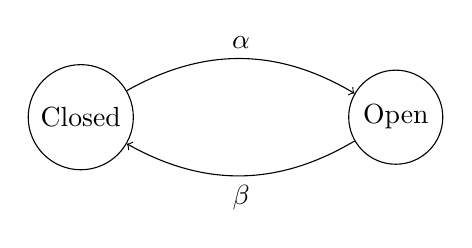
\begin{tikzpicture}[node distance=4cm, auto]
      % Nodes
      \node[draw, circle] (C) {Closed};
      \node[draw, circle, right of=C] (O) {Open};

      % Arrows
      \draw[->] (C) to[bend left] node[above] {$\alpha$} (O);
      \draw[->] (O) to[bend left] node[below] {$\beta$} (C);
    \end{tikzpicture}
    \caption{Transition diagram for the first-order kinetic model of gating variables}
    \label{fig:gating_first_order_kinetics}
\end{figure}

The functions for $x_\infty$ and $\tau_x$, as well as exponents $p$ and $q$ are generally derived from voltage-clamp recordings, while the maximal conductance is typically chosen to fit the model output to the experimental data.

Equation \ref{eq:differential_gating_steadyst_timeconst} is sometimes written as
\begin{equation}\label{eq:differential_gating_steadyst_timeconst_q10}
    \frac{dx}{dt} = \phi_x\frac{x - x_{\infty}}{\tau_x}
\end{equation}
to account for the temperature factor. $\phi_x$ is called $Q10$ value and is defined as \parencite{sterrattQ10EffectTemperature2015}:
\begin{equation}
    \phi_x=\frac{\text{Rate of process at temperature $T+10^\circ$C}}{\text{Rate of process at temperature $T$}}
\end{equation}

The equations \ref{eq:differential_gating_wtr_rates} and \ref{eq:differential_gating_steadyst_timeconst} describe first-order kinetics, with one open and one
closed state. However, to account for more complex gating behaviour, higher-order kinetics have been proposed that incorporate multiple open and/or closed states and diverse transition pathways
between them (see e.g. \parencite{wangModelTtypeCalcium1991,brunoUsingIndependentOpentoclosed2005}).

Finally, Equation \ref{eq:conductance_wrt_gating_variables} assumes that, in the case of multiple activation and/or inactivation gates, they exhibit similar kinetics (reflected in the use of the exponents $p$ and $q$). However, some studies have proposed models in which different gates are characterized by different time constants to capture more complex dynamics (see e.g. \parencite{destexheModelInwardCurrent1993}).


%%%%%%%%%%%%%%%%%%%%%%%%%%%%%%%%%%%%%%%%%%%%%%%%%%%%%%%%%%%%%%%%%%%%%%%%%%%%%%%%%
\subsection{Oscillations after \glsentrytext{ttx} Application} \label{subsec:math_backg_ttx_oscillations}

As shown Section \ref{subsubsec:experiment_ttx_t_type_block}, after Na$^+$ channels were blocked
R5 neurons exhibited slow oscillations likely mediated by Ca$^{2+}$ channels. The width of the spikes ($\sim 100$ms) was observed to be considerably smaller than interspike intervals ($\sim 2$s).
Such dynamics may arise through one of the following mechanisms: during the interspike interval
\begin{enumerate}
    \item the trajectory may pass near the bifurcation of equilibria (Hopf of \gls{snic}), where time derivatives of all variables are close to $0$, or
    \item the system consists of fast and slow subsystems, and the trajectory evolves along the slow manifold, where the fast subsystem is at equilibria while the slow subsystem gradually drives the system toward the spiking threshold.
\end{enumerate}

Such slow oscillations have been reported when the trajectory passes near a Hopf bifurcation \parencite{doiGenerationVerySlow2005}. However, the authors showed that the oscillation period depends exponentially on the injected current. Such behaviour is expected, as such dynamics require a specific intersection of the nullclines, and a slight deviation may significantly affect the dynamics. Similarly, near \gls{snic} bifurcation the oscillation period varies as $\sqrt{\lambda}$, where $\lambda$ is the distance from the bifurcation \parencite{strogatzNonlinearDynamicsChaos2018,izhikevichNEURALEXCITABILITYSPIKING2000} (see also Table \ref{tab:bifurcations_equilibria}). In both cases, slight variations in the external input can cause large changes in the oscillation period. However, such large variations in the oscillation period were not observed in the experiments. This suggests that in order to exhibit robustness to noise and small parameter variations, the system likely involves a slow variable operating on an ultra-slow timescale (order of seconds).

Apart from slow oscillations, the spikes after blockade of Na$^+$ channels showed apparent \gls{ahp} (see Sections \ref{subsubsec:ion_channel_contributions} and \ref{subsubsec:experiment_ttx_t_type_block}). Such undershoots of the membrane potential below the quasi-resting state have been associated with the h-current, mediated by \gls{hcn} channels \parencite{oswaldIHCurrentGenerates2009,boninHyperpolarizationActivatedCurrentIh2013}. However, the presence of these channels is not a necessary condition for \gls{ahp}. As depicted in Figure \ref{fig:potential_undershoot_izhikevich}, the presence of undershoot depends on the location of the two attractors of the dynamical system - the limit cycle and (quasi) stable equilibrium.

\begin{figure}[!t]
    \centering
    \includegraphics[width=0.85\linewidth]{../img/2_mathematical_overview/spike_undershoot_bw.png}
    \caption[Projection of the limit cycle and resting state on the voltage axis.]{
        \textbf{Projection of the limit cycle and resting state on the voltage axis.} 
        The spike undershoot depends on the location of the limit cycle attractor and (quasi) stable equilibrium of the dynamical system.
        Adapted from \parencite{izhikevichNEURALEXCITABILITYSPIKING2000}, with modifications.
    }
    \label{fig:potential_undershoot_izhikevich}
\end{figure}

%%%%%%%%%%%%%%%%%%%%%%%%%%%%%%%%%%%%%%%%%%%%%%%%%%%%%%%%%%%%%%%%%%%%%%%%%%%%%%%%%
% \subsection{Considerations for Modeling R5 Neurons}

% \color{red}

% As it was discussed in Section \ref{sec:sleep_and_r5_network}, \gls{swa} is thought to be generated at the level of R5 neurons. Thus, out of 4 bursting classes based on response to external current (\textcolor{red}{see Section ???}), R5 neurons may be either tonic, or inhibition-induced bursting neurons.

% (Okay, so, if Ca concentration affects the bursting, maybe one should model Ca dependent channels with Goldman-Hodgkin-Katz flux equation ??? It is even second argument for this equation, the first one being that the fit is better!!!) (Liu et al 2016)

% The paper about slow negative feedback: transition between the spiking and bursting requires slow positive feedback, thus, the activation function of T-Type current should NOT be instantaneous!!!

% Bifurcation analysis helpful for: explaining why neuron stays for short period in bursting?
% Why it is robust to perturbations or noise?

% \color{green}

% In Section \ref{subsubsec:math_bursting_classification} it was discussed, that based on the response to the external stimulus bursting neurons can be categorized into one of the four classes.
% Two out of these classes exhibit single, while the other two - repetitive bursts.
% As oscillations are considered to emerge within R5 neurons, out of the 4 bursting classes mentioned above, R5 neurons may be either tonic, or inhibition-induced bursting neurons (Figure \ref{fig:classification_intrin_burst}).

% From a dynamical systems perspective, bursting can arise through a variety of
% mechanisms, including stable limit cycles, chaotic attractors, canard-induced
% mixed-mode oscillations, and other complex nonlinear dynamics.

% Reduced system 2+1 or 2+2 - mostly studied, however one can accumulate all small timescales together (citation)

% Tuning parameters is generally hard, as there are many parameters (cite from that paper which fitted with that algorythm). Especially, in cases when the activation and inactivation curves overlay - changing one might affect everything. As many parameter regimes might lead to the same voltage trace, finding one parameter set that acts like R5 neuron might not be the same as it is in R5. Thus, for now, one could think of possible mechanisms that are model-independent. This might give us an insight which ion channels important in Drosophila R5 modulation.

% Thus, for starters, we would take already existing models and see if there is a common mechanism of spiking to bursting transition etc, that also aligns with the experimental findings discussed in Section biological background.

% Then, to get towards R5 model one should know the parameters for the ion channels of interest.

% \color{black}

% %%%%%%%%%%%%%%%%%%%%%%%%%%%%%%%%%%%%%%%%%%%%%%%%%%%%%%%%%%%%%%%%%%%%%%%%%%%%%%%%%

\end{document}